\chapter{Related Works}\label{ch:related_works}
This thesis builds upon prior research in knowledge graph fact verification, \ac{LLMs}, \ac{RAG}, and entailment verification.
In this section, we provide an overview of the relevant literature across these areas.

\section{Entailment Verification and Language Models}\label{sec:entailment-verification}
In the paper "Minds versus Machines: Rethinking Entailment Verification with Language Models", Sanyal et al.~\cite{sanyal2024machinesbettercomplexreasoning} evaluate and compare the inference capabilities of humans and \ac{LLMs} through a carefully constructed entailment verification benchmark.
Their study spans three categories: \ac{NLI}, contextual \ac{QA}, and rationales, using multi-sentence premises and diverse types of knowledge to assess inference across complex reasoning scenarios.

The authors found that LLMs generally excel in multi-hop reasoning tasks, particularly those requiring inference over extended contexts, while humans outperform \ac{LLMs} in simpler deductive reasoning tasks involving substitutions or negations.


\begin{figure}[ht!]
    \centering
    \begin{minipage}[b]{\textwidth}
        \centering
        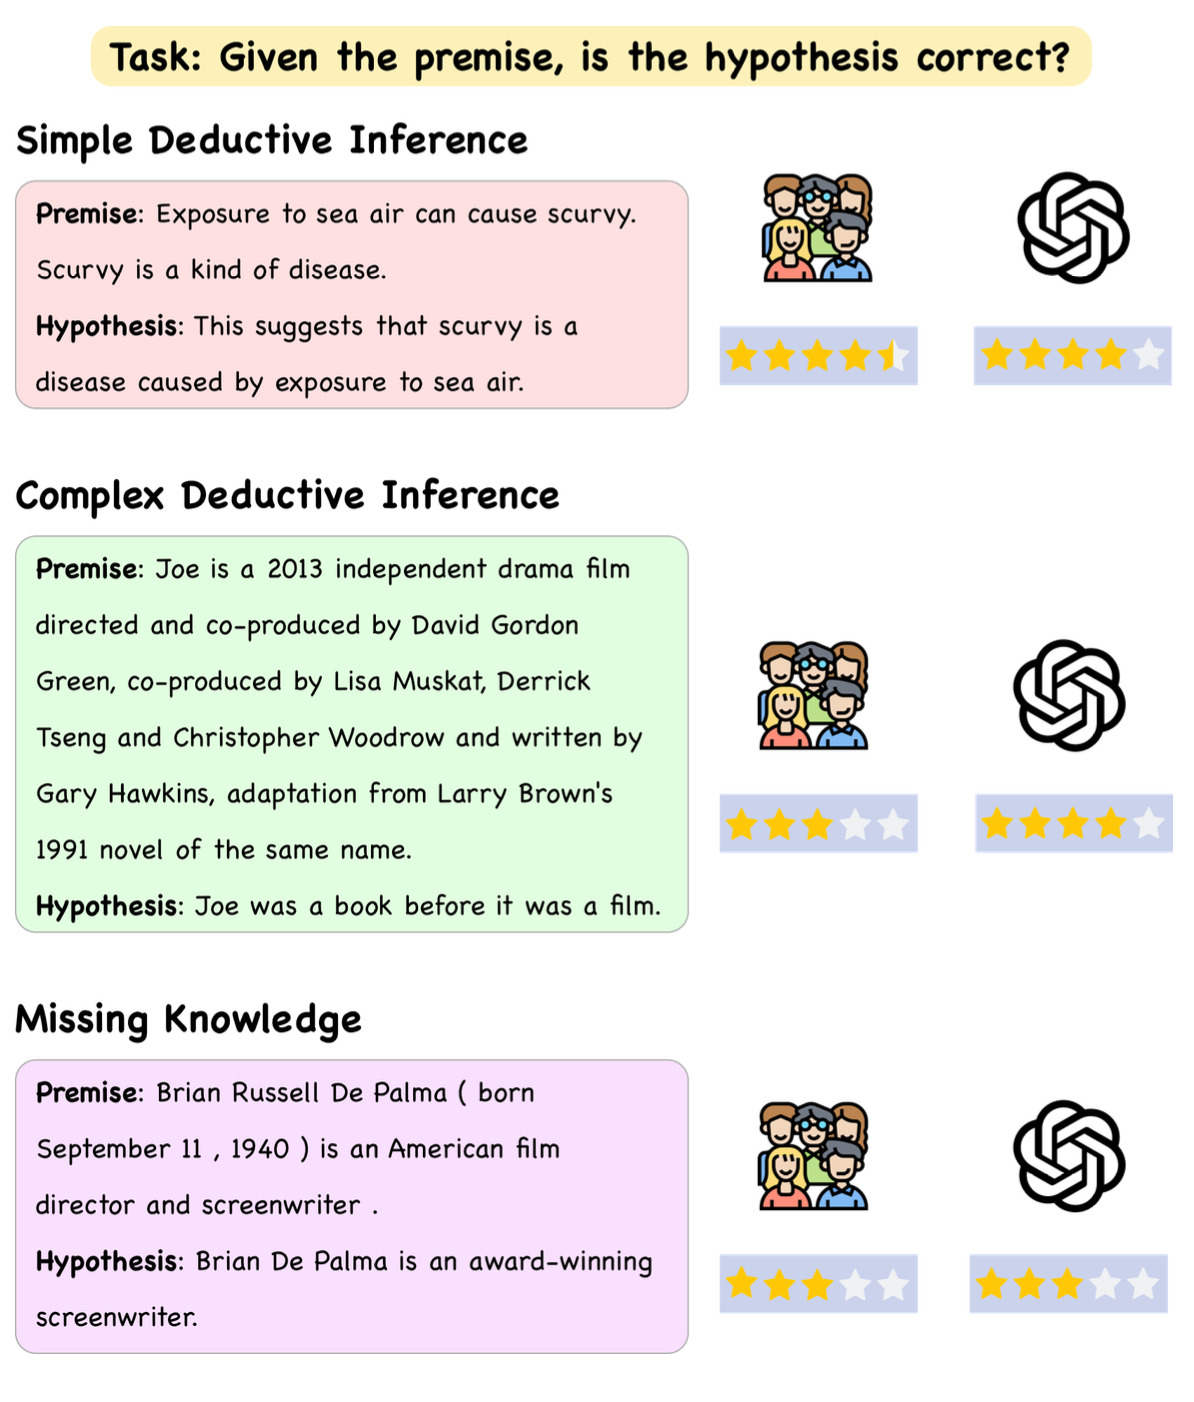
\includegraphics[width=0.6\textwidth]{res/rel-human-llm-inference}
        \caption{\textbf{Distinctions between human and LLM Inferences.} The entailment prediction performance of humans and LLMs are depicted by a 5-star rating scale~\cite{sanyal2024machinesbettercomplexreasoning}.}
        \label{fig:distinguishing-human-llm-inferences}
    \end{minipage}
\end{figure}

Interestingly, both perform comparably in situations requiring inference of missing knowledge.
One of the paper's key contributions is the fine-tuning of the Flan-T5~\cite{https://doi.org/10.48550/arxiv.2210.11416} model, which outperforms GPT-3.5 and performs at a comparable level to GPT-4, thus providing a robust, open-source solution for entailment verification tasks.
In contrast, the proposed approach to factulizing the knowledge graph using \ac{RAG} emphasizes the integration of external knowledge retrieval to ground factual assertions, which is critical for generating verifiable, accurate knowledge graphs.
While Sanyal et al. focus on the entailment between premises and hypotheses in textual inference, my work extends this by incorporating external evidence to ensure not just consistency but also factual correctness.

In comparison, the entailment verification tasks handled by Sanyal et al. emphasize reasoning within the constraints of the given context, whereas my \ac{RAG}-based approach highlights the necessity of retrieval from large external datasets to mitigate hallucinations and improve the factual grounding of generated content.
Both approaches deal with inference verification but diverge in their method of contextualizing and validating knowledge, with mine incorporating real-time retrieval for fact-checking.

This distinction is significant in terms of application: while their fine-tuned Flan-T5 model achieves high accuracy in entailment tasks, it remains bound to the contextual limits of its training data.
My work, by integrating retrieval, potentially overcomes this limitation by dynamically accessing external data, thus offering a complementary perspective to entailment verification focused on enhancing factuality.

\section{Claim Verification in the Age of Large Language Models}\label{subsec:claim-verification-in-the-age-of-large-language-models}
Dmonte et al.~\cite{dmonte2024claimverificationagelarge} provide a comprehensive survey ofc\ac{LLM}-based approaches to claim verification, highlighting the shift from traditional \ac{NLP} methods to more sophisticated LLM-driven techniques.

The typical LLM-based claim verification pipeline, as described by Dmonte et al., consists of several key components:
\begin{enumerate}
    \item Evidence Retrieval: Utilizing techniques like \ac{RAG} to fetch relevant information from external sources.
    \item Prompt Creation: Developing effective prompting strategies to guide LLMs in processing claims and evidence.
    \item Transfer Learning: Employing fine-tuning and in-context learning to adapt LLMs to the specific task of claim verification.
    \item LLM Generation: Using LLMs to generate veracity labels, supporting evidence, and explanations.
\end{enumerate}

This pipeline represents a departure from traditional fact-checking approaches, leveraging the power of \ac{LLMs} to improve accuracy and provide more nuanced assessments of claim veracity.

Several studies have demonstrated the effectiveness of LLM-based approaches in claim verification:
\begin{itemize}
    \item Zhang and Gao~\cite{zhang2024reinforcementretrievalleveragingfinegrained} introduced HiSS, a hierarchical prompting technique that improved performance on complex news claim verification tasks.
    \item Lee et al.~\cite{lee2023factualityenhancedlanguagemodels} developed FactualityPrompts, a framework for assessing the factual accuracy of LLM-generated content.
\end{itemize}

These studies consistently show that LLM-based methods outperform traditional NLP approaches in terms of accuracy, flexibility, and the ability to handle complex claims.

\begin{figure}[ht!]
    \centering
    \begin{minipage}[b]{\textwidth}
        \centering
        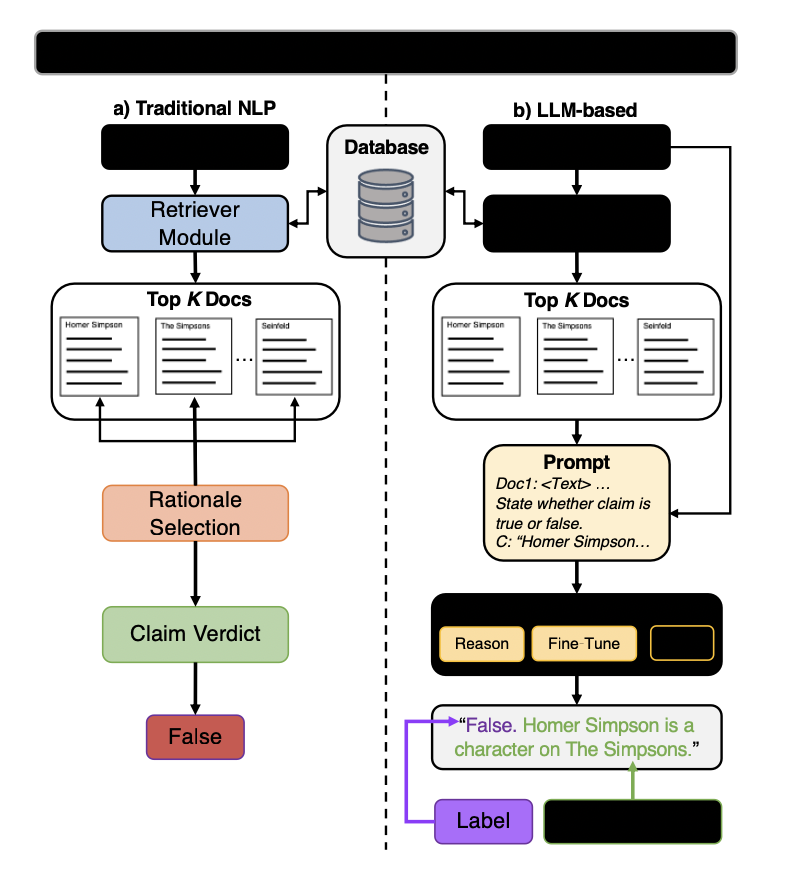
\includegraphics[width=0.6\textwidth]{res/rel-claim-verification}
        \caption{Comparison of claim verification systems between NLP-based (traditional) and LLM-based for claim veracity.~\cite{dmonte2024claimverificationagelarge}.}
        \label{fig:claim-verification-llm}
    \end{minipage}
\end{figure}

Our approach shares similarities with the LLM-based pipeline described by Dmonte et al., particularly in the use of retrieval-augmented generation and the integration of multiple LLMs. However, our method differs in several key aspects:
\begin{enumerate}
    \item Multi-Query Retrieval: We employ a multi-query strategy for evidence retrieval, potentially improving the coverage and relevance of supporting information.
    \item Iterative Refinement: Our system incorporates an iterative process for refining retrieved evidence and generated responses, which is not explicitly mentioned in most LLM-based approaches surveyed.
    \item Explainability Focus: While many LLM approaches provide explanations, our method places a stronger emphasis on generating detailed, step-by-step justifications for veracity assessments.
    \item Specialized Embedding Models: We utilize domain-specific embedding models for improved semantic understanding in the retrieval phase, which is not commonly discussed in general LLM-based approaches.
\end{enumerate}

These distinctions position our work as a novel contribution to the field, building upon the foundations of LLM-based claim verification while introducing innovative techniques to enhance performance and interpretability.

Despite the promising results of LLM-based claim verification, several challenges remain.
Dmonte et al. highlight issues such as handling irrelevant context, resolving knowledge conflicts, and expanding to multilingual settings. Our approach attempts to address some of these challenges, particularly in the areas of context relevance and explainability. However, there is still significant room for improvement in creating more robust, reliable, and universally applicable claim verification systems.

\section{Retrieval-Augmented Fact Verification by Synthesizing Contrastive Arguments}\label{sec:retrieval-augmented-fact-verification}
The paper Retrieval-Augmented Fact Verification by Synthesizing Contrastive Arguments~\cite{yue2024retrievalaugmentedfactverification} explores a method for improving fact verification in knowledge graphs using RAG.
The proposed framework combines retrieval of external information and the generation of contrastive arguments—claims supported by retrieved evidence, but also those that provide counterpoints.
This dual synthesis provides a richer and more nuanced verification process, allowing the system to handle conflicting evidence more effectively.
The core contribution of the work lies in the creation of contrastive arguments, a strategy designed to reduce errors in fact verification systems, especially when LLMs may hallucinate or generate incomplete reasoning.

The authors leverage a multi-stage pipeline where external documents are retrieved to support or refute a given claim.
Each retrieved piece of evidence is evaluated using a neural network model that ranks the evidence based on its relevance to the claim.
By synthesizing contrastive arguments, the system generates explanations for both supporting and refuting the claim, which helps improve the transparency and trustworthiness of the model's decisions.

\begin{figure}[ht!]
    \centering
    \begin{minipage}[b]{\textwidth}
        \centering
        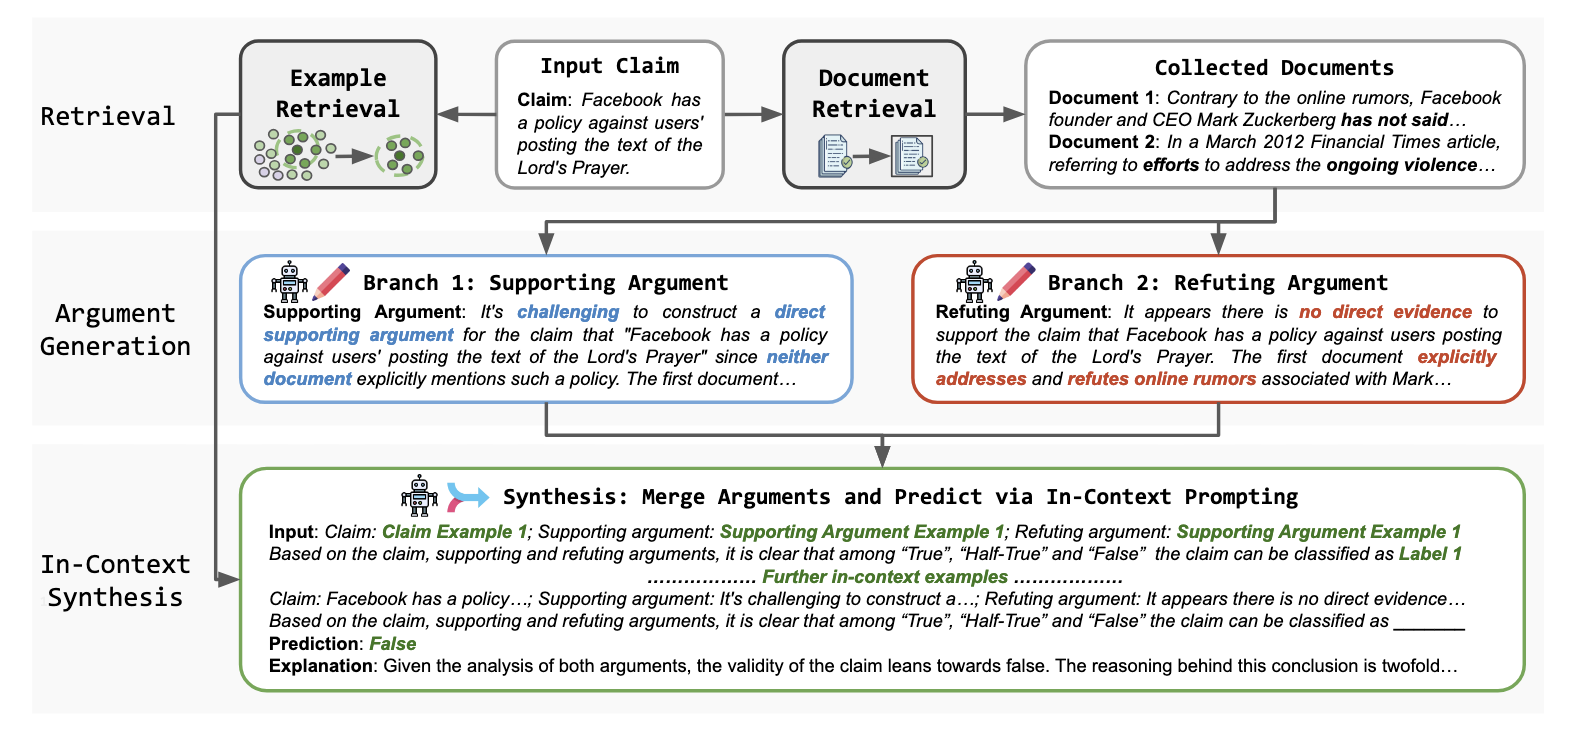
\includegraphics[width=\textwidth]{res/rel-rafts}
        \caption{The proposed RAFTS~\cite{yue2024retrievalaugmentedfactverification}, which performs few-shot fact verification by incorporating informative in-context demonstrations and contrastive arguments with nuanced information derived from the retrieved documents}
        \label{fig:rel-rafts}
    \end{minipage}
\end{figure}

In terms of results, the framework shows improvement over traditional fact verification pipelines, particularly in handling ambiguous or conflicting information.
The contrastive arguments allow for better handling of cases where facts are not binary but exist in a more complex, nuanced state.
The system's ability to generate arguments for both sides of a claim increases its robustness and provides a more reliable fact verification tool.

The described approach and my work on fact verification in knowledge graphs using RAG share a common goal: improving the factual accuracy of information through the integration of external knowledge retrieval.
However, there are key differences in the methodologies used.
The contrastive argument synthesis introduced by the authors focuses heavily on generating both supporting and opposing arguments for claims, which provides a more holistic perspective in scenarios where evidence is mixed.
In contrast, my approach emphasizes majority voting among multiple models and a multi-query strategy to retrieve a broader range of external evidence, aiming to reduce the incidence of hallucinations in LLM outputs.

While both approaches use retrieval to mitigate the limitations of LLMs, my work incorporates adaptive dispute resolution techniques and focuses on synthesizing outputs from multiple LLMs rather than generating contrastive arguments.
This means that my approach leans more towards optimizing model diversity and utilizing the best consensus from several LLMs to ensure factual accuracy, rather than explicitly generating opposing arguments for each claim.

\section{RAGAR: RAG-Augmented Reasoning for Political Fact-Checking using Multimodal LLMs}\label{sec:agar-rag-augmented-reasoning}
The study titled RAGAR: RAG-Augmented Reasoning for Political Fact-Checking using Multimodal LLMs~\cite{khaliq2024ragarfalsehoodradarragaugmented} introduces a novel approach to political fact-checking by leveraging RAG with multimodal LLMs.
This work focuses on enhancing fact verification in the politically sensitive domain, where disinformation can have far-reaching consequences.
The authors integrate various modalities text, images, and other media sources into a unified fact-checking pipeline powered by LLMs, particularly emphasizing RAG’s ability to retrieve and synthesize external evidence to validate or refute claims.

\begin{figure}[ht!]
    \centering
    \begin{minipage}[b]{\textwidth}
        \centering
        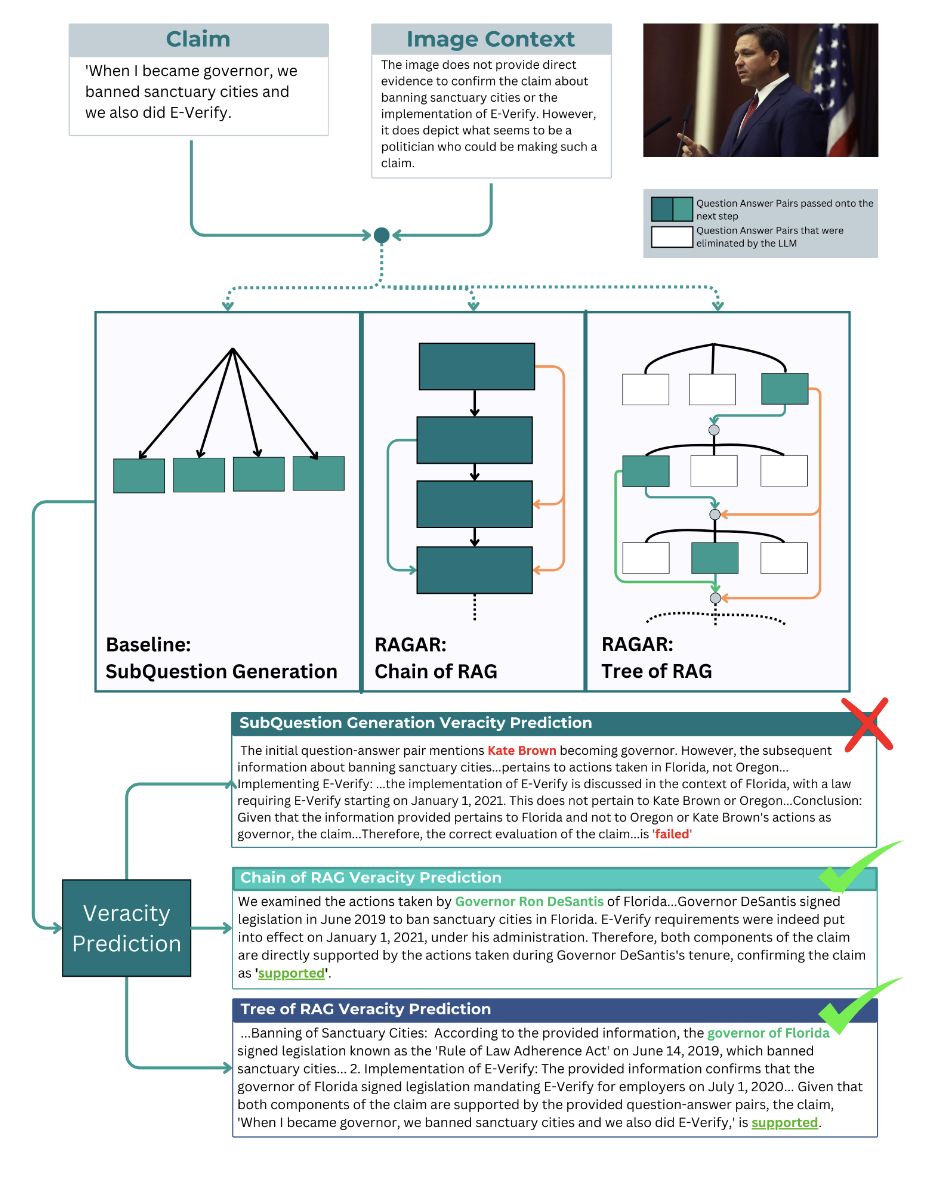
\includegraphics[width=0.6\textwidth]{res/rel-ragar}
        \caption{An overview of the fact-checking pipeline~\cite{khaliq2024ragarfalsehoodradarragaugmented} contrasting the baseline Sub-Question Generation approach from the RAGAR: Chain of RAG and RAGAR: Tree of RAG approach followed by a veracity explanation generated by a Veracity Prediction module.}
        \label{fig:rel-ragar}
    \end{minipage}
\end{figure}

The central innovation of RAGAR lies in its multimodal reasoning capabilities, which allow the model to handle political claims that involve not only textual content but also visual data, such as images or charts.
By extending RAG to this multimodal context, the system improves its ability to assess the veracity of claims in real-time, leveraging external resources such as political databases and live web content.
Furthermore, the use of contrastive learning helps the system generate both supporting and opposing arguments for each claim, providing a more balanced and comprehensive fact-checking process.

Results from the paper show significant improvements in fact-checking accuracy, particularly for politically charged claims that are often more nuanced or context-dependent.
RAGAR's ability to synthesize multimodal evidence into a coherent verification report highlights its potential for real-world applications, especially in environments where disinformation spreads quickly, such as social media platforms.

RAGAR focuses on political fact-checking using multimodal data, whereas my work targets the factualization of knowledge graphs with a primary focus on textual information.
In contrast to RAGAR’s multimodal pipeline, my system emphasizes multi-query strategies and document chunking techniques to retrieve highly relevant textual evidence for verification.

% TODO: ADD FUTURE WORK